% ----------------------------------------------------------
\chapter{Algoritmos e estruturas de dados para consulta de pontos no plano}\label{cap:desenvolvimento}
% ----------------------------------------------------------
Nesta seção veremos formas de construir estruturas de dados para um conjunto de pontos no plano. 
Consideramos que os pontos são fixos. Para cada estrutura construída, veremos também como utilizá-la para
consultar pontos dentro de uma janela.

% ----------------------------------------------------------
\section{Árvore KD}
% ----------------------------------------------------------

Uma árvore KD é uma árvore binaria onde cada folha é um ponto \textit{k-dimensional}.
Cada nó não-folha é um valor $v$ em uma dimensão $d$, representando implicitamente um hiperplano.
Pontos cujo os valores na dimensão $d$ são iguais ou menores a $v$ estão na subárvore da esquerda de $v$,
e respectivamente, pontos maiores que $v$ estão para o lado direito.
Cada nó é associado com uma das \textit{k dimensões}. Então, a citar um exemplo no plano, se dado nó
 divide o eixo
$x$, a subárvore a esquerda contem os pontos com o eixo $x$ menor que o ponto de corte. Similarmente,
 ã direita contem
os pontos com o eixo $x$ maior que o ponto de corte. 

\begin{figure}[htb]
    \caption{\label{fig:Fig_1}Árvore \textit{3-dimensional}}
    \begin{center}
        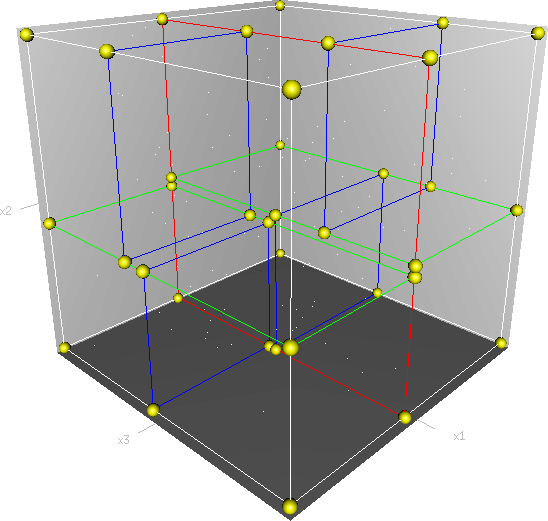
\includegraphics[width=\linewidth/2]{./images/3dtree.png}
    \end{center}
    \fonte{GPL}
\end{figure}

\subsection{Arvore 2D}
Uma árvore 2D é a versão com duas dimensões para árvores KD.

A construção de uma árvore 2D pode ser feita da seguinte forma.
É dado um conjunto $P$ de $n$ pontos no plano.

Uma consulta 2-dimensional em $P$ é uma busca de quais pontos de $P$ da busca estão
entre um retângulo de consulta \([x,x']  \times  [y,y']\). 
Um ponto $p:= (p_x, p_y)$ está dentro de um retângulo de busca se e somente se:

\[
p_x \in [x, x'] \textrm{ e } p_y \in [y, y`]
\]

Podemos dizer que uma consulta 2-dimensional é composta de duas sub-consultas 1-dimensional: uma no
eixo \(x\) de um dos pontos e uma consulta no eixo \(y\).

\begin{figure}[htb]
    \caption{\label{fig:Fig_2}Busca em alcance \textit{dimensional} - 2D}
    \begin{center}
        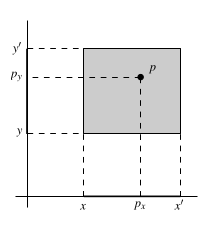
\includegraphics{images/search_range.png}
    \end{center}
\end{figure}

\subsection{Construção da Árvore 2-dimensional}
Na construção de uma árvore para 2 dimensões, cada ponto tem uma forma $P : (P_x, P_y)$ .
Escolhemos um eixo para iniciar a construção da árvore. Ao iniciar a construção da arvore,
ordenamos os pontos de $P$ pelo eixo escolhido. A ordenação acontecerá ao menos $n$ dimensões
vezes, uma vez em cada eixo.
O \cite{cg08} valor da mediana dos pontos ordenados pelo eixo será o valor de corte do conjunto $P$,
e serão criados dois subconjuntos.
Chama-se recursivamente a construção das subárvores ã esquerda e ã direita de $v$ alternando o eixo 
e passando os subconjuntos.

\begin{figure}[htb]
    \caption{\label{fig:Fig_3} Árvore 2D}
    \begin{center}
        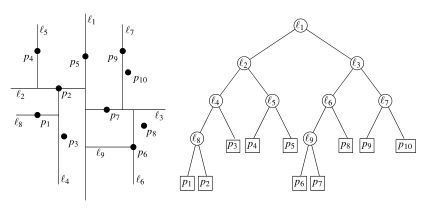
\includegraphics{images/kd_tree1.png}
    \end{center}
\end{figure}


Seja $P$ conjunto de pontos. Inicialmente escolhemos o eixo-$x$. Acompanharemos a troca de eixos 
segundo a profundidade da árvore.
Caso a profundidade seja $par$, ordenaremos pelo eixo $x$, do contrário pelo eixo $y$.
Fazemos uma $x$-ordenação em $P$ e encontramos o valor $x_{mediana}$.
Criamos dois subconjuntos $P_1$ e $P_2$ tal que:
    \[P_1 \leftarrow p : p \in P \textmd{ e } p_x \leq x_{mediana} \]
    \[P_2 \leftarrow p : p \in P \textmd{ e } p_x  >  x_{mediana} \]
Agora, recursivamente, repete-se para os dois novos conjuntos criados até restar somente um ponto.
 Este, por sua vez, será um nó folha.

\begin{algorithm}
    \caption{O algorítimo \Call{ConstroiArvore2D}{$P$, $profundidade=0$}, recebe um conjunto de 
    pontos $P$ no plano e uma profundidade da árvore.
    O algoritmo retorna a raiz de uma árvore 2D}
    \begin{algorithmic}[1]
        \Function{ConstroiArvore2D}{$P$, $profundidade$}
            \If{P contem apenas um ponto}
            \Return $nó \leftarrow ponto$
        \Else
            \If{$profundidade$ é par}
            \State
                Divide P em dois subconjuntos com um linha vertical $l$ pela mediana da $x$-coordenada
                dos pontos em P. Seja $P_1$ o conjunto dos pontos à esquerda de $l$ e seja
                $P_2$ o conjunto de pontos à direita de $l$.
            \Else
            \State
                Divide P em dois subconjuntos com um linha horizontal $l$ pela mediana da $y$-coordenada
                dos pontos em P. Seja $P_1$ o conjunto dos pontos abaixo de $l$ e seja
                $P_2$ o conjunto de pontos acima de $l$.
            \EndIf
        \EndIf
        \State Cria os nós $v_{esquerda}$ e $v_{direita}$
        \State $v_{esquerda} \leftarrow $ \Call{ConstroiArvore2D}{$P_1, profundidade+1$}
        \State $v_{direita} \leftarrow $ \Call{ConstroiArvore2D}{$P_2, profundidade+1$}
        \State Cria um nó $v$, associamos o valor $l$ e associamos os filhos $v_{esquerda}$ e $v_{direita}$ 

        \Return $v$
        \EndFunction
    \end{algorithmic}
\end{algorithm}

\subsection{Consulta}

Agora retomamos para o algoritmo de consulta. Podemos supor que os pontos na subárvore à esquerda
da raiz, possuindo $x$-coordenada no máximo igual ao valor de $l_1$ armazenado na raiz.
Enquanto os pontos na subárvore à direita do nó raiz possuem $x$-coordenada maior que $l_1$.

A exemplo: a região correspondente do nó \(l_4\) é limitada à esquerda de
\(l_1\) e abaixo \(l_2\).


\begin{figure}[htb]
    \caption{\label{fig:Fig_4} Área respectiva do nó $l_4$}
    \begin{center}
        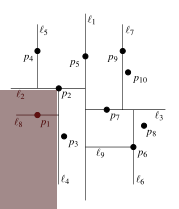
\includegraphics{images/kd_tree2.png}
    \end{center}
\end{figure}

Denotaremos esta área de um nó \(v\) como \(região(v)\). A região da raiz é (no caso de uma árvore 2D) 
o plano inteiro.
Portanto, o algoritmo buscará pela subárvore com raiz \(v\) somente se o retângulo de busca intersectar
a \(região(v)\).

O algoritmo de busca funciona descendo a árvore, mas visitando somente os nós que a
\(região(v)\) intersecta o retângulo da consulta. Quando uma \(região(v)\) está contida na
janela de busca devolvemos todos os pontos na subárvore.
Quando chegarmos nos nós folha temos de checar se o nodo esta dentro da consulta, se estiver,
devolvê-lo.

Segue o algoritmo que recebe como parâmetros a raiz da arvore2D e o retângulo de consulta \(R\).
Usamos uma chamada \(RetornaSubárvore(v)\) que atravessa a árvore do nó \(v\) e retorna
todos os pontos nas suas folhas. Segue como notação \(filho_{esquerda}(v)\) sendo o filho da esquerda e
\(filho_{direita}(v)\) o filho da direita do nó \(v\).


\begin{algorithm}
    \caption{A função \Call{BuscaEmArvore2D}{$v$, $consulta$} recebe como parâmetro um nó e uma 
    consulta.
     E retorna todos os pontos dentro da consulta.}
    \begin{algorithmic}[1]
    \Function{BuscaEmArvore}{$v$, $consulta$}
        \If{v é folha}
        \Return  $v$ se estiver dentro da $consulta$
        \Else
            \If{$região(filho_{esquerda}(v))$ está contido na $consulta$}
            \State \Return $Subárvore( filho_{esquerda}(v) )$
            \Else
                \If{$região(filho_{esquerda}(v))$ intersecta $consulta$}
                \State \Call{BuscaEmArvore2D}{$filho_{esquerda}(v)$, $consulta$}
                \EndIf
            \EndIf
            \If{$região(filho_{direita}(v))$ está contido na $consulta$}
            \State \Return $Subárvore(filho_{direita}(v))$
            \Else
                \If{$região(filho_{direita}(v))$ intersecta $busca$}
                \State \Call{BuscaEmArvore2D}{$filho_{direita}(v)$, $consulta$}
                \EndIf
            \EndIf
        \EndIf
    \EndFunction
    \end{algorithmic}
\end{algorithm}

A comparação realizada é checar se a área \(consulta\) intersecta a região
de um nodo \(v\). Para isso precisamos computar \(região(v)\) para todos os nodos \(v\)
durante a fase de construção da árvore.
Uma alternativa é manter a região salva nas chamadas recursivas usando as linhas guardadas
nos nodos internos. Por exemplo, a região correspondente ao filho esquerda de um nodo
\(v\) em uma profundidade par (no exemplo 2D, analisamos no eixo \(x\)) pode ser calculado com:
\[
    região(filho_{esquerda}(v)) = região(v) \cap l(v)^{esquerda}
\]
onde \(l(v)\) é a linha que divide o eixo salvo em \(v\), e \(l(v)^{esquerda}\) é a metade
esquerda do plano.
Mantendo apenas os intervalos respectivos de cada nível da árvore. 

\section{Resultados}
\begin{figure}[htb]
    \caption{\label{fig:Fig_5} — Resultados de busca com Arvore2D}
    \begin{center}
        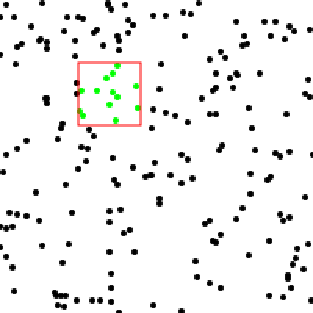
\includegraphics{images/points.pdf}
    \end{center}
\end{figure}


Na Figura 5 temos os pontos:

(70.0, 73.0), (-10.0, 24.0), (0.0, 0.0), (-44.0, 39.0), (-49.0, 3.0), (15.0, 56.0), 
(-9.0, -44.0), (23.0, 21.0), (-43.0, -13.0), (-6.0, -13.0), (18.0, 31.0), (8.0, -19.0),
 (24.0, 13.0)

E a consulta (o retângulo em vermelho) as coordenadas: (-50, -10), (50, 40), (-50, 40), (50, -10)

Retornando corretamente o conjunto de pontos:

(-49.0, 3.0),
(-44.0, 39.0),
(-10.0, 24.0),
(0.0, 0.0),
(18.0, 31.0),
(23.0, 21.0),
(24.0, 13.0)

Sendo facilmente verificável apenas constatando que os valores $x$:
\[ x \leq 50 \textrm{ e } x > -50 \]
\[ y \leq 10 \textrm{ e } y > -10 \]

\section{Arvore de Intervalos}
% ----------------------------------------------------------

% ----------------------------------------------------------